\documentclass[a4paper,
fontsize=11pt,
%headings=small,
oneside,
numbers=noperiodatend,
parskip=half-,
bibliography=totoc,
final
]{scrartcl}

\usepackage[babel]{csquotes}
\usepackage{synttree}
\usepackage{graphicx}
\setkeys{Gin}{width=.8\textwidth} %default pics size

\graphicspath{{./plots/}}
\usepackage[ngerman]{babel}
\usepackage[T1]{fontenc}
%\usepackage{amsmath}
\usepackage[utf8x]{inputenc}
\usepackage [hyphens]{url}
\usepackage{booktabs} 
\usepackage[left=2.4cm,right=2.4cm,top=2.3cm,bottom=2cm,includeheadfoot]{geometry}
\usepackage[labelformat=empty]{caption} % option 'labelformat=empty]' to surpress adding "Abbildung 1:" or "Figure 1" before each caption / use parameter '\captionsetup{labelformat=empty}' instead to change this for just one caption
\usepackage{eurosym}
\usepackage{multirow}
\usepackage[ngerman]{varioref}
\setcapindent{1em}
\renewcommand{\labelitemi}{--}
\usepackage{paralist}
\usepackage{pdfpages}
\usepackage{lscape}
\usepackage{float}
\usepackage{acronym}
\usepackage{eurosym}
\usepackage{longtable,lscape}
\usepackage{mathpazo}
\usepackage[normalem]{ulem} %emphasize weiterhin kursiv
\usepackage[flushmargin,ragged]{footmisc} % left align footnote
\usepackage{ccicons} 
\setcapindent{0pt} % no indentation in captions
\usepackage{xurl} % Breaks URLs

%%%% fancy LIBREAS URL color 
\usepackage{xcolor}
\definecolor{libreas}{RGB}{112,0,0}

\usepackage{listings}

\urlstyle{same}  % don't use monospace font for urls

\usepackage[fleqn]{amsmath}

%adjust fontsize for part

\usepackage{sectsty}
\partfont{\large}

%Das BibTeX-Zeichen mit \BibTeX setzen:
\def\symbol#1{\char #1\relax}
\def\bsl{{\tt\symbol{'134}}}
\def\BibTeX{{\rm B\kern-.05em{\sc i\kern-.025em b}\kern-.08em
    T\kern-.1667em\lower.7ex\hbox{E}\kern-.125emX}}

\usepackage{fancyhdr}
\fancyhf{}
\pagestyle{fancyplain}
\fancyhead[R]{\thepage}

% make sure bookmarks are created eventough sections are not numbered!
% uncommend if sections are numbered (bookmarks created by default)
\makeatletter
\renewcommand\@seccntformat[1]{}
\makeatother

% typo setup
\clubpenalty = 10000
\widowpenalty = 10000
\displaywidowpenalty = 10000

\usepackage{hyperxmp}
\usepackage[colorlinks, linkcolor=black,citecolor=black, urlcolor=libreas,
breaklinks= true,bookmarks=true,bookmarksopen=true]{hyperref}
\usepackage{breakurl}

%meta
%meta

\fancyhead[L]{P. Falkenburg\\ %author
LIBREAS. Library Ideas, 44 (2023). % journal, issue, volume.
\href{https://doi.org/10.18452/28265}{\color{black}https://doi.org/10.18452/28265}
{}} % doi 
\fancyhead[R]{\thepage} %page number
\fancyfoot[L] {\ccLogo \ccAttribution\ \href{https://creativecommons.org/licenses/by/4.0/}{\color{black}Creative Commons BY 4.0}}  %licence
\fancyfoot[R] {ISSN: 1860-7950}

\title{\LARGE{Praxisbericht institutionalisiertes Grassroots Open Access : Beitrag der Vernetzungs- und Kompetenzstelle Open Access Brandenburg (VuK) zum Open Access Tracking Project (OATP)}}% title
\author{Philipp Falkenburg} % author

\setcounter{page}{1}

\hypersetup{%
      pdftitle={Praxisbericht institutionalisiertes Grassroots Open Access : Beitrag der Vernetzungs- und Kompetenzstelle Open Access Brandenburg (VuK) zum Open Access Tracking Project (OATP)},
     pdfauthor={Philipp Falkenburg},
      pdfcopyright={CC BY 4.0 International},
      pdfsubject={LIBREAS. Library Ideas, 44 (2023).},
      pdfkeywords={OATP, Community-basierte Verschlagwortung, Vernetzungs- und Kompetenzstelle Open Access Brandenburg, community tagging},
      pdflicenseurl={https://creativecommons.org/licenses/by/4.0/},
      pdfurl={https://doi.org/10.18452/28265},
      pdfdoi={10.18452/28265},
      pdflang={de},
      pdfmetalang={de}
     }



\date{}
\begin{document}

\maketitle
\thispagestyle{fancyplain} 

%abstracts

%body
\hypertarget{vernetzungs--und-kompetenzstelle-open-access-brandenburg}{%
\section{Vernetzungs- und Kompetenzstelle Open Access
Brandenburg}\label{vernetzungs--und-kompetenzstelle-open-access-brandenburg}}

Mit der Verabschiedung der Open-Access-Strategie des Landes
Brandenburg\footnote{\url{https://doi.org/10.5281/zenodo.3757920}} am 8.
August 2019 verpflichtete sich das Land Brandenburg unter anderem zur
Einrichtung einer Landesstelle zur Unterstützung der acht durch das
Ministerium für Wissenschaft, Forschung und Kultur geförderten
Hochschulen bei der Open-Access-Transformation. Im Anschluss an zwei
Vorprojekte zur Konzeption und zur Bedarfsabschätzung zu
Open-Access-spezifischen Kompetenzen an den Hochschulbibliotheken nahm
die \emph{Vernetzungs- und Kompetenzstelle Open Access Brandenburg
(VuK)}\footnote{\url{https://open-access-brandenburg.de/}} zum 1. April
2021 die Arbeit auf. Die Arbeitsaufgaben der VuK reichen von
Strategieberatung über Informationsvermittlung, Einrichtung und Betrieb
eines landesweiten Publikationsfonds für Open-Access-Monografien, Aufbau
und Durchführung eines Open-Access-Monitorings für Brandenburg bis zur
Koordination und Vernetzung der Community. Dafür stehen aktuell zwei
Vollzeitstellen zur Verfügung. Der Aufbau der VuK und ihrer Teilprojekte
erfolgen agil und unter Berücksichtigung der immer wieder spontan
aufkommenden Bedarfe aus den Einrichtungen und der
Open-Access-Community. So ist es auch nur folgerichtig, dass die VuK
inzwischen auch als Anknüpfungspunkt für weitere Spin-off-Projekte, wie
das im September dieses Jahres gestartete Projekt \enquote{Kulturwandel
in der Rechtswissenschaft} (KidRewi),\footnote{\url{https://kidrewi.de},
  siehe auch Hantow, Jonas: Projektstart: KidRewi öffnet Türen für mehr
  Open Access in der Rechtswissenschaft. In: open-access-brandenburg.de
  / Newsblog.
  \url{https://open-access-brandenburg.de/projektstart-kidrewi-oeffnet-tueren-fuer-mehr-open-access-in-der-rechtswissenschaft/}}
fungiert. Momentan wird die VuK evaluiert und aktiv weiterentwickelt.

Im vorliegenden Beitrag wird eine besondere Facette des auf die
Open-Access-Community gerichteten Engagements der VuK beleuchtet: das
Einpflegen von Quellen und Publikationen zum Thema Open Access aus dem
Umfeld der VuK in das \enquote{Open Access Tracking Projekt}.

\hypertarget{open-access-tracking-projekt}{%
\section{Open Access Tracking
Projekt}\label{open-access-tracking-projekt}}

Das \enquote{Open Access Tracking Projekt} (OATP) ist ein von Peter
Suber\footnote{\url{https://de.wikipedia.org/wiki/Peter_Suber}}
gegründetes Projekt zur Verschlagwortung von Webinhalten zum Themenfeld
Open Access. Besonderheiten des Projekts sind, dass es auf einem rein
Community-basierten Ansatz (\emph{crowd-sourced}) aufbaut und die
verschlagwortenden Personen nicht speziell geschult oder ausgebildet
sein müssen (\emph{social tagging}).\footnote{Suber, Peter: The open
  access tracking project (OATP). In: SPARC Open Access Newsletter,
  issue \#133. May 02, 2009.
  \url{http://nrs.harvard.edu/urn-3:HUL.InstRepos:4322586}} Lediglich
ein Set von grundlegenden Konventionen\footnote{Diese und weitere
  Informationen wie FAQ sind im Wiki des Projekts nachzulesen:
  \url{https://cyber.harvard.edu/hoap/Open_Access_Tracking_Project}}
sollte beim sogenannten \emph{Taggen} eingehalten werden. Technisch baut
der Dienst auf der von der Harvard University entwickelten (ebenfalls
unter der Leitung von Peter Suber) und betriebenen
Social-Tagging-Plattform TagTeam\footnote{\url{https://cyber.harvard.edu/research/tagteam}}
auf. OATP ist auf TagTeam ein sogenannter \emph{Hub}. Team-Hubs sind
abgegrenzte Bereiche, in denen die jeweiligen Teams kollaborativ Tags
für ihre Inhalte zusammenstellen.\footnote{\url{https://cyber.harvard.edu/hoap/TagTeam_FAQ\#How_do_I_create_a_TagTeam_hub.3F}}
Die Hubs sind grundsätzlich öffentlich.\footnote{\url{https://cyber.harvard.edu/hoap/TagTeam_FAQ\#How_do_I_create_a_private_hub_or_use_private_tags.3F}}

Bezüglich der Inhalte gibt es neben dem Themenbezug zu Open Access und
der Anforderung, dass die Inhalte per URL auffindbar sein müssen, keine
weiteren Einschränkungen -- kreative Arbeiten, Stellenangebote,
Veranstaltungshinweise, aber natürlich auch Publikationen über Open
Access sowie alle weiteren denkbaren Inhalte sind ausdrücklich
gewünscht.\footnote{Suber, Peter: The open access tracking project
  (OATP). In: SPARC Open Access Newsletter, issue \#133. May 02, 2009.
  \url{http://nrs.harvard.edu/urn-3:HUL.InstRepos:4322586}}

Der Nutzen von OATP ergibt sich aus der Präsentation der getaggten
Inhalte: Alle verschlagworteten Inhalte (\emph{items}) werden
chronologisch im sogenannten \emph{main feed} dargestellt, aber jedes
\emph{Tag} für sich wird ebenfalls in einem getrennten Feed abgebildet.
Die einzelnen Feeds können so nach individuellen Vorlieben oder
Anforderungen abonniert (RSS, ATOM, JSON) werden -- analog eines
klassischen Alertdienstes. Einmal ins System aufgenommene Items sind
aber nicht statisch, sondern können jederzeit um weitere Tags ergänzt
werden -- und dies von allen am Projekt teilnehmenden Konten, wodurch
das auf der Plattform kumulierte Wissen fortwährend um weitere
Informationen oder Zuordnungen angereichert wird.

Der Weg zur aktiven Teilnahme an OATP ist dabei denkbar einfach und
erfordert lediglich vier Schritte:\footnote{Ausführliche Anleitung mit
  Links unter:
  \url{https://cyber.harvard.edu/hoap/Get_started_as_a_tagger}}

\begin{enumerate}
\def\labelenumi{\arabic{enumi}.}
\item
  Erstellung eines TagTeam-Accounts,
\item
  Freischaltung für OATP,
\item
  Einrichtung eines Tagging-Bookmarks im Browser,
\item
  Kenntnisnahme (und Einhaltung!) der Konventionen.\footnote{\url{https://cyber.harvard.edu/hoap/OATP_conventions}}
\end{enumerate}

Die OATP-Schlagworte sind grundlegend nach dem Muster
\emph{oa.{[}tag{]}} aufgebaut. Neben einigen vorgegebenen und vielen
durch erstmalige Verwendung angelegten Tags ist es auch möglich, eigene
Tags zu kreieren und dadurch eigene Communitys abzubilden -- so hat die
VuK beispielsweise den Tag oa.vuk eingeführt und durch kontinuierliche
Nutzung inhaltlich befüllt. Durch das Tagging-Bookmark wird die
Oberfläche zum Erfassen und Editieren aufgerufen, über die neben den
Tags eine Reihe weiterer Metadaten angegeben werden. Einige dieser
Felder werden automatisch aus den Informationen der jeweiligen Webseite
vorausgefüllt (zum Beispiel das Feld Titel und URL). Unabhängig von der
Sprache der jeweiligen Ressource soll bei jeder Verschlagwortung eine
kurze Beschreibung in englischer Sprache beigefügt werden, was dank
Übersetzungstools wie DeepL\footnote{\url{https://www.deepl.com/de/translator}}
schnell erledigt ist.

\begin{figure}
\centering
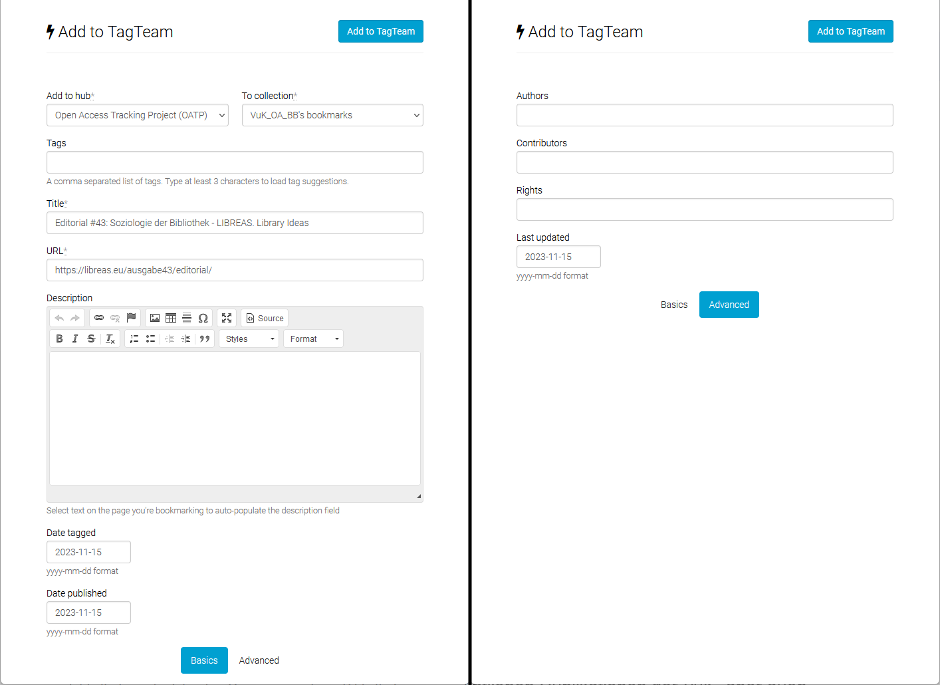
\includegraphics{img_1.png}
\caption{Über das Tagging-Bookmark aufgerufene Seite zur
Verschlagwortung und Angabe weiterer Metadaten.}
\end{figure}

\hypertarget{vuk-x-oatp}{%
\section{VuK x OATP}\label{vuk-x-oatp}}

Die Vernetzungs- und Kompetenzstelle Open Access Brandenburg wirkt neben
ihren offiziellen Aufgaben aktiv auch an
Grassroots-Open-Access-Projekten wie OATP mit. So werden monatlich die
jeweils veröffentlichen Publikationen der VuK, aber auch
Veröffentlichungen zum Thema Open Access aus dem Land Brandenburg von
der VuK per OATP verschlagwortet. Diese Arbeit integriert sich in
bestehende Workflows zur Sicherung eigener Inhalte und wird durch eine
studentische Hilfskraft des Projekts durchgeführt. Der Umfang dieser
Tätigkeit beläuft sich pro Monat aktuell auf ungefähr zwei Stunden --
sie ist aber stark vom Aufkommen der zu verschlagwortenden Inhalte
abhängig und kann somit für andere Institutionen variieren.

Da sich die VuK selbst noch im Status der Erprobung des Dienstes
befindet, ist die Verschlagwortungstiefe bisher nicht sonderlich hoch.
Die durch die VuK meistgenutzten \emph{tags} sind aktuell oa.vuk (unser
eigener Tag für Inhalte von uns), oa.new (für Inhalte, die in den
letzten sechs Monaten erschienen sind), oa.german (für Inhalte auf
Deutsch) und oa.germany (für Inhalte aus Deutschland).

\begin{figure}
\centering
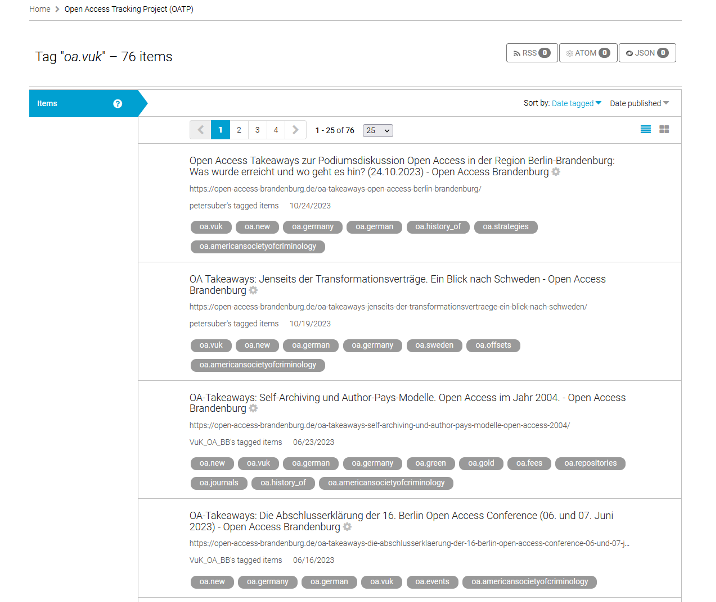
\includegraphics{img_2.png}
\caption{Screenshot der Übersicht des Tags oa.vuk.}
\end{figure}

\hypertarget{macht-mit}{%
\section{Macht mit!}\label{macht-mit}}

Bibliotheken und andere Informationseinrichtungen verwalten nicht nur
Wissen und Informationen im Auftrag von oder für
Wissenschaftscommunitys, sondern sind immer auch Teil dieser Communitys.
Als den Prinzipien des Open Access verpflichtete Einrichtungen sollten
sie insbesondere auch Ansätze wahrnehmen, welche \emph{community-driven}
sind, diese bewerben und sich aktiv im Rahmen ihrer Möglichkeiten
beteiligen. Die Open-Access-Bewegung als Ganzes ist immer nur so stark
wie das Engagement der sich einbringenden Anhänger*innen zusammen
genommen. Neben rein idealistischen Beweggründen zur Teilnahme stellt
ein solches Engagement immer auch einen kommunikativen Mehrwert für die
jeweilige Institution und ein gelebtes Bekenntnis zu Open Access als
solches dar.

Jede weitere \emph{taggende} Person oder Institution würde das Projekt
und die Open-Access-Community stärken und den Transformationsprozess ein
kleines Stück voranbringen. Zugleich schreibt sich eine teilnehmende
Institution selbst sichtbar und dadurch auch vorbildhaft in diesen
Gesamtkatalog der Open-Access-Aktivitäten ein.

\emph{Die Anregung wurde auch in die Redaktion der LIBREAS eingebracht
und dort gerne aufgenommen.}

%autor
\begin{center}\rule{0.5\linewidth}{0.5pt}\end{center}

\textbf{Philipp Falkenburg} (https://orcid.org/0000-0001-9788-8277) hat
Philosophie, Soziologie und Bibliothekswissenschaft studiert und
letzteres im Herbst 2023 an der Fachhochschule Potsdam abgeschlossen
(BA). Zurzeit ist er wissenschaftlicher Mitarbeiter der Vernetzungs- und
Kompetenzstelle Brandenburg und im BMBF-Projekt KidRewi -- Kulturwandel
in der Rechtswissenschaft. Außerdem ist er seit 2022 Mitglied der
Redaktion LIBREAS.Library Ideas.

\end{document}